%% ═══════════════════════════════════════════════════════════════════════════
%% PCEOT503: POWER SYSTEMS — MODULE 1 COMPREHENSIVE STUDY MATERIAL
%% APJ Abdul Kalam Technological University / CET S5 (2024 Scheme)
%% Styled with Anthropic Notes Design System — Complete Line-by-Line Edition
%% ═══════════════════════════════════════════════════════════════════════════

\documentclass[11pt,a4paper]{article}

%% ─── Packages ────────────────────────────────────────────────────────────────
\usepackage{fontspec}

%% Font configuration with local fonts and synthetic fallbacks
\setmainfont{Anthropic-serif}[
    Path          = ./,
    Extension     = .ttf,
    AutoFakeBold  = 1.5,
    AutoFakeSlant = 0.2
]
\setsansfont{Poppins}[
    AutoFakeBold  = 1.5,
    AutoFakeSlant = 0.2
]
\setmonofont{DejaVu Sans Mono}[Scale=MatchLowercase]

\usepackage[margin=2.0cm, top=2.5cm, bottom=2.5cm, headheight=25pt]{geometry}
\usepackage[table]{xcolor}
\usepackage{tikz}
\usetikzlibrary{shapes.geometric, arrows.meta, positioning, fit, backgrounds,
                decorations.pathreplacing, calc, patterns}
\usepackage{listings}
\usepackage{tcolorbox}
\tcbuselibrary{listings, skins, breakable, raster}
\usepackage{fancyhdr}
\usepackage{titlesec}
\usepackage{titletoc}
\usepackage{enumitem}
\usepackage{booktabs}
\usepackage{tabularx}
\usepackage{array}
\usepackage{microtype}
\usepackage{hyperref}
\usepackage{amssymb}
\usepackage{amsmath}
\usepackage{parskip}
\usepackage{colortbl}

%% ─── Document Metadata ──────────────────────────────────────────────────────
\newcommand{\docsubject}{PCEOT503: Power Systems (S5 EEE)}
\newcommand{\docshortsubject}{PCEOT503 · Mod 1}
\newcommand{\doctitle}{Generation, Storage \& Load Dynamics}
\newcommand{\docauthor}{Sudheesh}

%% ─── Widow / Orphan Protection ──────────────────────────────────────────────
\widowpenalty=10000
\clubpenalty=10000

%% ─── Spacing ────────────────────────────────────────────────────────────────
\setlength{\parskip}{0.45em plus 0.15em minus 0.1em}
\setlength{\parindent}{0pt}

%% ─── Table Geometry ─────────────────────────────────────────────────────────
\setlength{\aboverulesep}{0pt}
\setlength{\belowrulesep}{0pt}
\setlength{\extrarowheight}{0.65ex}
\renewcommand{\arraystretch}{1.4}
\setlength{\arrayrulewidth}{0.4pt}

\newcolumntype{L}[1]{>{\raggedright\arraybackslash}p{#1}}
\newcolumntype{C}[1]{>{\centering\arraybackslash}p{#1}}
\newcolumntype{R}[1]{>{\raggedleft\arraybackslash}p{#1}}

%% ─── Brand Colors (Anthropic Palette) ────────────────────────────────────────
\definecolor{AnthDark}{HTML}{141413}
\definecolor{AnthLight}{HTML}{faf9f5}
\definecolor{AnthMidGray}{HTML}{7a7870}
\definecolor{AnthLightGray}{HTML}{e8e6dc}
\definecolor{AnthOrange}{HTML}{d97757}
\definecolor{AnthBlue}{HTML}{3b75a4}
\definecolor{AnthGreen}{HTML}{5d7343}
\definecolor{AnthCodeBG}{HTML}{edebe1}
\definecolor{AnthCardBG}{HTML}{f6f5ee}

\arrayrulecolor{AnthMidGray!40}

%% ─── Hyperref ────────────────────────────────────────────────────────────────
\hypersetup{
  colorlinks  = true,
  linkcolor   = AnthBlue,
  urlcolor    = AnthOrange,
  citecolor   = AnthGreen,
  pdftitle    = {\doctitle{} · \docsubject},
  pdfauthor   = {\docauthor},
}

%% ─── Page Style ─────────────────────────────────────────────────────────────
\pagestyle{fancy}
\fancyhf{}
\fancyhead[L]{\small\sffamily\color{AnthMidGray}\textbf{\doctitle} \textbar\ \docshortsubject}
\fancyhead[R]{\small\sffamily\color{AnthMidGray}\thepage}
\renewcommand{\headrulewidth}{0.4pt}
\renewcommand{\headrule}{%
  \hbox to\headwidth{\color{AnthOrange}\leaders\hrule height \headrulewidth\hfill}}
\renewcommand{\footrulewidth}{0.4pt}
\renewcommand{\footrule}{%
  \hbox to\headwidth{\color{AnthLightGray}\leaders\hrule height \footrulewidth\hfill}}
\fancyfoot[L]{\footnotesize\sffamily\color{AnthMidGray} APJ Abdul Kalam Technological University (KTU S5 EEE)}
\fancyfoot[R]{\footnotesize\sffamily\color{AnthMidGray} PCEOT503 Study Material}

%% ─── Section Formatting ─────────────────────────────────────────────────────
\titleformat{\section}
  {\Large\bfseries\sffamily\color{AnthDark}}
  {\colorbox{AnthOrange}{\makebox[0.65cm][c]{\color{white}\thesection}}\quad}
  {0em}
  {}
  [\vspace{-0.5ex}\color{AnthLightGray}\hrule\vspace{0.4ex}]

\titleformat{\subsection}
  {\large\bfseries\sffamily\color{AnthDark}}
  {\color{AnthBlue}\thesubsection\enspace}
  {0em}{}

\titleformat{\subsubsection}
  {\normalsize\bfseries\sffamily\color{AnthDark}}
  {\color{AnthGreen}\thesubsubsection\enspace}
  {0em}{}

\titlespacing{\section}     {0pt}{1.5em}{0.6em}
\titlespacing{\subsection}  {0pt}{1.1em}{0.3em}
\titlespacing{\subsubsection}{0pt}{0.8em}{0.25em}

%% ─── Table of Contents Styling ──────────────────────────────────────────────
\contentsmargin{0pt}

\titlecontents{section}
  [0pt]
  {\vspace{4pt}\bfseries\sffamily\color{AnthDark}}
  {\colorbox{AnthOrange}{\makebox[0.55cm][c]{\color{white}\small\thecontentslabel}}\enspace}
  {}
  {\hfill\color{AnthOrange}\contentspage}

\titlecontents{subsection}
  [1.5em]
  {\small\sffamily\color{AnthBlue}}
  {\thecontentslabel\enspace}
  {}
  {\titlerule*[6pt]{\tiny\color{AnthMidGray}.}\color{AnthBlue}\contentspage}

\titlecontents{subsubsection}
  [3.5em]
  {\footnotesize\sffamily\color{AnthGreen}}
  {\thecontentslabel\enspace}
  {}
  {\titlerule*[6pt]{\tiny\color{AnthMidGray}.}\color{AnthGreen}\contentspage}

%% ─── tcolorbox Styles ───────────────────────────────────────────────────────
\tcbset{
  notebox/.style={
    enhanced, breakable,
    colback     = AnthCardBG,
    colframe    = AnthMidGray,
    arc=4pt, outer arc=4pt,
    sharp corners=west,
    left=9pt, right=9pt, top=7pt, bottom=7pt,
    boxrule     = 0.5pt,
    colupper    = AnthDark,
    fonttitle   = \bfseries\sffamily\small,
    coltitle    = AnthDark,
    colbacktitle= AnthLightGray,
    borderline west={3pt}{0pt}{AnthMidGray},
    drop fuzzy shadow={AnthMidGray!20},
  },
  tipbox/.style={
    enhanced, breakable,
    colback     = AnthGreen!8,
    colframe    = AnthGreen!70,
    arc=4pt, outer arc=4pt,
    sharp corners=west,
    left=9pt, right=9pt, top=7pt, bottom=7pt,
    boxrule     = 0.5pt,
    colupper    = AnthDark,
    fonttitle   = \bfseries\sffamily\small,
    coltitle    = white,
    colbacktitle= AnthGreen,
    borderline west={3pt}{0pt}{AnthGreen},
    drop fuzzy shadow={AnthGreen!20},
  },
  warnbox/.style={
    enhanced, breakable,
    colback     = AnthOrange!7,
    colframe    = AnthOrange!70,
    arc=4pt, outer arc=4pt,
    sharp corners=west,
    left=9pt, right=9pt, top=7pt, bottom=7pt,
    boxrule     = 0.5pt,
    colupper    = AnthDark,
    fonttitle   = \bfseries\sffamily\small,
    coltitle    = white,
    colbacktitle= AnthOrange,
    borderline west={3pt}{0pt}{AnthOrange},
    drop fuzzy shadow={AnthOrange!20},
  },
  defbox/.style={
    enhanced, breakable,
    colback     = AnthLight,
    colframe    = AnthLightGray,
    arc=4pt, outer arc=4pt,
    sharp corners=west,
    left=9pt, right=9pt, top=7pt, bottom=7pt,
    boxrule     = 0.5pt,
    colupper    = AnthDark,
    borderline west={3.5pt}{0pt}{AnthOrange},
    drop fuzzy shadow={AnthMidGray!20},
  },
  problembox/.style={
    enhanced, breakable,
    colback     = AnthBlue!6,
    colframe    = AnthBlue!80,
    arc=4pt, outer arc=4pt,
    sharp corners=west,
    left=9pt, right=9pt, top=7pt, bottom=7pt,
    boxrule     = 0.5pt,
    colupper    = AnthDark,
    fonttitle   = \bfseries\sffamily\small,
    coltitle    = white,
    colbacktitle= AnthBlue,
    borderline west={3.5pt}{0pt}{AnthBlue},
    drop fuzzy shadow={AnthBlue!20},
  },
  solbox/.style={
    enhanced, breakable,
    colback     = AnthLight,
    colframe    = AnthGreen!60,
    arc=4pt, outer arc=4pt,
    sharp corners=west,
    left=9pt, right=9pt, top=7pt, bottom=7pt,
    boxrule     = 0.5pt,
    colupper    = AnthDark,
    fonttitle   = \bfseries\sffamily\small,
    coltitle    = white,
    colbacktitle= AnthGreen!85,
    borderline west={3.5pt}{0pt}{AnthGreen},
    drop fuzzy shadow={AnthGreen!15},
  }
}

%% ─── Inline Helpers & Custom Environments ────────────────────────────────────
\newcommand{\ic}[1]{\mbox{\colorbox{AnthCodeBG}{\footnotesize\ttfamily\textcolor{AnthBlue}{#1}}}}

\newcommand{\concept}[1]{%
  \vspace{3pt}\noindent\textcolor{AnthGreen}{\rule{3.5pt}{10pt}}\enspace
  \textbf{\sffamily\color{AnthDark}#1}\par\vspace{2pt}%
}

\newcommand{\syllabusitem}[1]{%
  \begin{tcolorbox}[enhanced, colback=AnthOrange!8, colframe=AnthOrange, boxrule=0.4pt, arc=3pt, left=7pt, right=7pt, top=3pt, bottom=3pt]
    \small\sffamily\textbf{\color{AnthOrange}Syllabus Requirement:} #1
  \end{tcolorbox}
}

\newenvironment{Note}[1][Note]{\begin{tcolorbox}[notebox, title=#1]}{\end{tcolorbox}}
\newenvironment{Tip}[1][Key Engineering Insight]{\begin{tcolorbox}[tipbox, title=#1]}{\end{tcolorbox}}
\newenvironment{Warn}[1][Important Exam Alert]{\begin{tcolorbox}[warnbox, title=#1]}{\end{tcolorbox}}
\newenvironment{Def}[1][]{\begin{tcolorbox}[defbox]\ifx&#1&\else\textbf{\color{AnthOrange}#1:}\enspace\fi}{\end{tcolorbox}}
\newenvironment{Problem}[1][Numerical Problem]{\begin{tcolorbox}[problembox, title=#1]}{\end{tcolorbox}}
\newenvironment{Solution}[1][Step-by-Step Solution]{\begin{tcolorbox}[solbox, title=#1]}{\end{tcolorbox}}

%% ─── Lists Styling ──────────────────────────────────────────────────────────
\setlist[itemize,1]{itemsep=1.5pt, topsep=2pt, parsep=0pt, label={\color{AnthOrange}\small$\blacktriangleright$}}
\setlist[itemize,2]{itemsep=1.5pt, topsep=2pt, parsep=0pt, label={\color{AnthBlue}\small$\blacktriangleright$}}
\setlist[itemize,3]{itemsep=1.5pt, topsep=2pt, parsep=0pt, label={\color{AnthGreen}\small$\blacktriangleright$}}

\setlist[enumerate,1]{itemsep=1.5pt, topsep=2pt, parsep=0pt, label={\bfseries\color{AnthOrange}\arabic*.}}
\setlist[enumerate,2]{itemsep=1.5pt, topsep=2pt, parsep=0pt, label={\bfseries\color{AnthBlue}(\alph*)}}
\setlist[enumerate,3]{itemsep=1.5pt, topsep=2pt, parsep=0pt, label={\color{AnthGreen}\roman*.}}

%% ─── Title Page Macro ───────────────────────────────────────────────────────
\newcommand{\maketitlepage}{%
  \begin{titlepage}
    \pagecolor{AnthDark}
    \color{AnthLight}
    \vspace*{2.2cm}
    \begin{center}
      {\huge\bfseries\sffamily \doctitle}\\[0.8em]
      {\Large\sffamily\color{AnthOrange} \docsubject}\\[0.4em]
      {\large\sffamily\color{AnthMidGray} Bachelor of Technology (B.Tech) — 2024 Scheme}\\[2.0em]
      \color{AnthOrange}\rule{0.5\textwidth}{1.2pt}\\[1.8em]
      {\normalsize\sffamily\color{AnthLightGray} Comprehensive Study Notes \& Numerical Problem Solving Suite}\\[0.4em]
      {\small\sffamily\color{AnthMidGray} Prepared from Course Materials, Lecture Slides \& KTU Curriculum}\\[2.8em]
      \begin{tcolorbox}[enhanced, width=0.84\textwidth, colback=AnthDark!90, colframe=AnthOrange!60, arc=4pt, boxrule=0.6pt]
        \centering\small\sffamily\color{AnthLight}
        \textbf{Module 1 Complete Syllabus Coverage:}\\[3pt]
        $\bullet$ Conventional Sources: Hydroelectric, Thermal (Rankine, Brayton, CCPP), Nuclear\\
        $\bullet$ Variable Renewables: Solar PV, Solar Thermal (CSP), Wind Turbine Systems\\
        $\bullet$ Energy Storage Systems: BESS, CESS (CAES), Thermal Energy Storage (TES)\\
        $\bullet$ Environmental \& Ethical Factors, National \& Global Regulatory Policies\\
        $\bullet$ Load Curves, Load Duration Curves, Power Station Economics \& 12 Numerical Problems
      \end{tcolorbox}
      \vfill
      {\small\sffamily\color{AnthMidGray} Compiled \today}
    \end{center}
    \vspace*{0.8cm}
  \end{titlepage}
  \pagecolor{AnthLight}
  \color{AnthDark}
}

%% ═══════════════════════════════════════════════════════════════════════════
%% DOCUMENT BODY
%% ═══════════════════════════════════════════════════════════════════════════
\begin{document}

\maketitlepage

%% ─── Table of Contents ───────────────────────────────────────────────────────
\thispagestyle{empty}
{
  \hypersetup{hidelinks}
  \tableofcontents
}
\clearpage

%% ─────────────────────────────────────────────────────────────────────────────
\section{Conventional Power Generation Technologies}
%% ─────────────────────────────────────────────────────────────────────────────

\syllabusitem{Generation from renewable and non-renewable sources -- Hydro, thermal, nuclear -- (block schematic details, environmental and ethical factors, advantages, disadvantages)}

\subsection{Overview of Electrical Power Generation}

Electrical energy is a secondary energy carrier derived from primary resources found in nature. The global power system has historically relied on three proven conventional generation technologies:
\begin{enumerate}
  \item \textbf{Thermal Power Plants:} Convert the chemical energy of fossil fuels into heat, generating high-pressure, superheated steam that drives rotating steam turbines.
  \item \textbf{Hydroelectric Power Plants:} Convert the gravitational potential energy of water stored at elevated heads into mechanical and electrical power.
  \item \textbf{Nuclear Power Plants:} Exploit controlled nuclear fission chain reactions to release binding energy from atomic nuclei to generate steam.
\end{enumerate}

These conventional generation assets form the \textbf{baseload bedrock} of modern synchronous power grids due to their high availability, dispatchability, and inherent synchronous rotational inertia.

%% ─────────────────────────────────────────────────────────────────────────────
\subsection{Hydroelectric Power Plants}

\concept{Working Principle \& Energy Conversion}
A hydroelectric power plant utilizes the potential energy of water stored in an elevated reservoir. As water flows through closed pressurized conduits called \textbf{penstocks}, potential energy converts to kinetic energy. The resulting high-velocity water jet strikes the runner blades of a \textbf{hydraulic turbine}, converting hydraulic energy into rotational mechanical energy. An electromechanically coupled \textbf{synchronous generator} converts this mechanical torque into 3-phase AC electricity via electromagnetic induction.

\begin{Def}[Energy Conversion Chain in Hydroelectric Plants]
\begin{align*}
  \text{Gravitational Potential Energy} &\xrightarrow{\text{Penstock}} \text{Kinetic Energy} \\
  &\xrightarrow{\text{Hydraulic Turbine}} \text{Mechanical Energy} \xrightarrow{\text{Generator}} \text{Electrical Energy}
\end{align*}
The theoretical hydraulic power developed at the turbine shaft is given by:
\begin{equation}
  P = \rho \cdot g \cdot Q \cdot H \cdot \eta \quad \text{[Watts]}
\end{equation}
where $\rho = 1000\,\text{kg/m}^3$ (water density), $g = 9.81\,\text{m/s}^2$ (acceleration due to gravity), $Q$ is discharge volume rate ($\text{m}^3/\text{s}$), $H$ is the effective net head (m), and $\eta$ is overall plant efficiency.
\end{Def}

\concept{Block Schematic \& Major Plant Components}

\begin{center}
\resizebox{0.92\textwidth}{!}{%
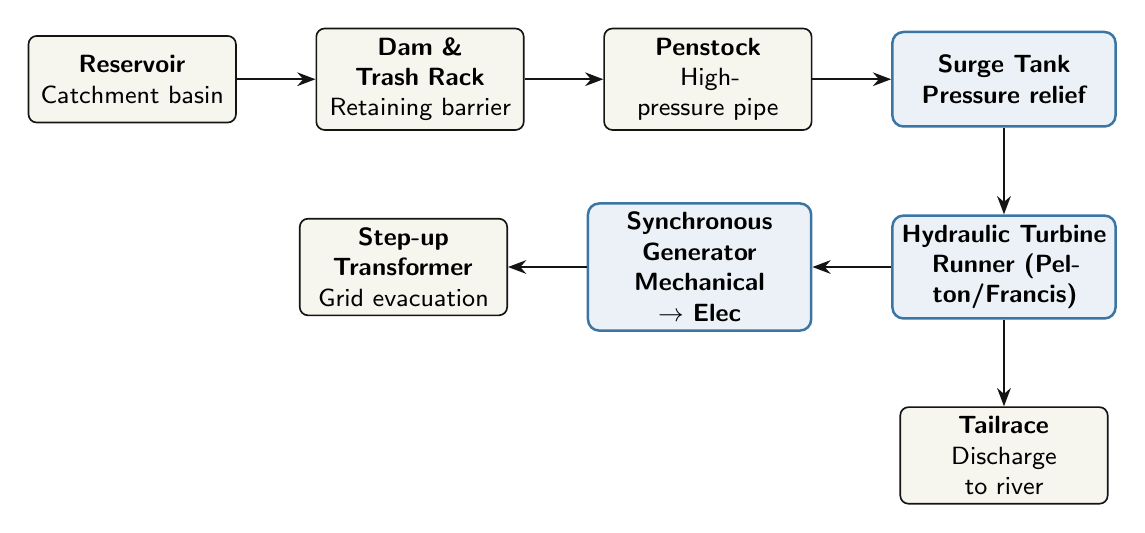
\begin{tikzpicture}[
  node distance=0.8cm and 1.0cm,
  block/.style={rectangle, draw=AnthDark, fill=AnthCardBG, rounded corners=3pt, line width=0.6pt, text width=2.4cm, align=center, minimum height=1.1cm, font=\small\sffamily},
  majorblock/.style={rectangle, draw=AnthBlue, fill=AnthBlue!10, rounded corners=4pt, line width=0.9pt, text width=2.6cm, align=center, minimum height=1.2cm, font=\small\sffamily\bfseries},
  arrow/.style={-{Stealth[scale=1.0]}, line width=0.8pt, color=AnthDark}
]
  \node[block] (res) {\textbf{Reservoir}\\ Catchment basin};
  \node[block, right=of res] (dam) {\textbf{Dam \& Trash Rack}\\ Retaining barrier};
  \node[block, right=of dam] (pen) {\textbf{Penstock}\\ High-pressure pipe};
  \node[majorblock, right=of pen] (st) {\textbf{Surge Tank}\\ Pressure relief};
  
  \node[majorblock, below=1.1cm of st] (turb) {\textbf{Hydraulic Turbine}\\ Runner (Pelton/Francis)};
  \node[majorblock, left=of turb] (gen) {\textbf{Synchronous Generator}\\ Mechanical $\to$ Elec};
  \node[block, left=of gen] (trans) {\textbf{Step-up Transformer}\\ Grid evacuation};
  \node[block, below=1.1cm of turb] (tail) {\textbf{Tailrace}\\ Discharge to river};

  \draw[arrow] (res) -- (dam);
  \draw[arrow] (dam) -- (pen);
  \draw[arrow] (pen) -- (st);
  \draw[arrow] (st) -- (turb);
  \draw[arrow] (turb) -- (gen);
  \draw[arrow] (gen) -- (trans);
  \draw[arrow] (turb) -- (tail);
\end{tikzpicture}%
}
\end{center}

\begin{enumerate}
  \item \textbf{Storage Reservoir:} Stores river water during high-inflow monsoon seasons to guarantee year-round operational supply.
  \item \textbf{Dam:} A civil engineering barrier (gravity, arch, or earth-rockfill) built across a river to create the required hydrostatic head.
  \item \textbf{Forebay \& Trash Racks:} Located at the penstock intake; screens prevent floating debris, tree branches, and silt from entering the pressurized pipe.
  \item \textbf{Penstock:} Heavy-walled steel or prestressed concrete conduits conveying high-pressure water from reservoir to turbine.
  \item \textbf{Surge Tank:} A vertical standing pipe or open shaft located on long penstocks near the powerhouse. It mitigates dangerous hydraulic pressure surges during sudden governor valve closures (\emph{water hammer effect}) and supplies supplemental water during sudden load pick-ups.
  \item \textbf{Hydraulic Turbine:} Extracts energy from moving water:
    \begin{itemize}
      \item \emph{Impulse Turbine (Pelton Wheel):} High head ($>300\,\text{m}$), low discharge rate.
      \item \emph{Reaction Turbine (Francis Turbine):} Medium head ($30-300\,\text{m}$), medium discharge rate.
      \item \emph{Axial Flow Turbine (Kaplan Turbine):} Low head ($<30\,\text{m}$), high discharge volume.
    \end{itemize}
  \item \textbf{Draft Tube:} An airtight diverging discharge pipe fitted to reaction turbines to recover kinetic exit energy.
  \item \textbf{Tailrace:} The exit channel discharging spent water back into the natural downstream river.
\end{enumerate}

\concept{Key Operational Features \& Real-World Benchmarks}
\begin{itemize}
  \item \textbf{Rapid Start-up \& Load Following:} Hydro units can ramp from complete standstill to 100\% rated power within 2 to 5 minutes, making them prime assets for \textbf{peak-load dispatch, spinning reserve, and grid black start}.
  \item \textbf{High Velocity Jets:} Water falling through large hydroelectric dams can exceed speeds of \textbf{$100\,\text{km/h}$} before striking the turbine runner.
  \item \textbf{Idukki Hydroelectric Project (Kerala):} Installed capacity $780\,\text{MW}$ ($6 \times 130\,\text{MW}$ Pelton units). Built across the Periyar River between the two granite hills \emph{Kuravan} and \emph{Kurathi}. It is India's first and one of Asia's largest double-curvature parabolic \textbf{arch dams} ($168.9\,\text{m}$ height), feeding an underground powerhouse at Moolamattom. During monsoon peaks, opening the spillway gates attracts thousands of visitors.
  \item \textbf{Tehri Dam (Uttarakhand):} India's tallest dam standing at $260.5\,\text{m}$ (similar in height to the Eiffel Tower), supplying $1,000\,\text{MW}$ of peaking power.
  \item \textbf{Three Gorges Dam (China):} The world's largest power station ($22,500\,\text{MW}$). In 2005, NASA scientist \textbf{Dr. Benjamin Fong Chao} calculated that when full ($39.3\times 10^9\,\text{m}^3$ of water mass), the Three Gorges reservoir shifted Earth's mass distribution enough to increase the length of a day by approximately \textbf{$0.06\,\mu\text{s}$}.
\end{itemize}

\begin{Note}[Advantages \& Disadvantages of Hydroelectric Power]
\textbf{Advantages:} Clean and renewable with zero operational greenhouse gas emissions; negligible operating costs (no fuel); long operating life ($>80-100\,\text{years}$); fast response for peak load and frequency control; provides multipurpose flood control and irrigation benefits.\\
\textbf{Disadvantages:} Very high upfront capital expenditure; long construction gestation periods (often $6-10\,\text{years}$); strict dependence on seasonal monsoon rains; geographically constrained to hilly terrain distant from load centers.
\end{Note}

\concept{Environmental \& Ethical Considerations}
\begin{itemize}
  \item \textbf{Environmental:} Inundation of vast forest and wildlife habitats; physical barrier to fish migration (partially mitigated by artificial \emph{fish ladders} or \emph{fish elevators}); anaerobic decay of submerged vegetation generating biogenic methane ($\text{CH}_4$); altered downstream sediment transport.
  \item \textbf{Ethical \& Social:} Involuntary resettlement of indigenous and rural populations; equitable compensation and livelihood rehabilitation; interstate and international river water-sharing disputes (e.g., Cauvery basin); submergence of cultural and historical heritage.
\end{itemize}

%% ─────────────────────────────────────────────────────────────────────────────
\subsection{Thermal Power Plants (Steam, Gas \& Combined Cycle)}

\concept{Working Principle \& Thermodynamic Cycles}
A thermal power plant converts the chemical energy of fuel into thermal energy to generate high-pressure, superheated steam that drives a steam turbine.

\begin{Def}[Energy Conversion Chain in Thermal Plants]
\begin{align*}
  \text{Chemical Energy (Fuel)} &\xrightarrow{\text{Combustion}} \text{Thermal Energy} \\
  &\xrightarrow{\text{Steam Turbine}} \text{Mechanical Energy} \xrightarrow{\text{Generator}} \text{Electrical Energy}
\end{align*}
\end{Def}

\concept{Thermodynamic Classifications}
\begin{enumerate}
  \item \textbf{Steam Power Plant (Rankine Cycle):} Water/steam circulates in a closed loop undergoing pressurized heating, evaporation, multi-stage turbine expansion, condensation, and pumping.
  \item \textbf{Gas Turbine Power Plant (Brayton Cycle):} Compressed air is mixed with natural gas or diesel in a combustor, and expanding hot combustion gases directly rotate a gas turbine ($10-15\,\text{min}$ quick start for peaking duty).
  \item \textbf{Combined Cycle Power Plant (CCPP):} Integrates a gas turbine (\emph{Brayton topping cycle}) with a steam turbine (\emph{Rankine bottoming cycle}). Hot exhaust gases ($>500^\circ\text{C}$) pass through a \textbf{Heat Recovery Steam Generator (HRSG)} to generate steam for a second turbine, achieving overall efficiencies \textbf{exceeding 60\%} (compared to $35-42\%$ for standalone steam cycles).
\end{enumerate}

\concept{Block Schematic of a Coal-Fired Thermal Power Plant}

\begin{center}
\resizebox{0.95\textwidth}{!}{%
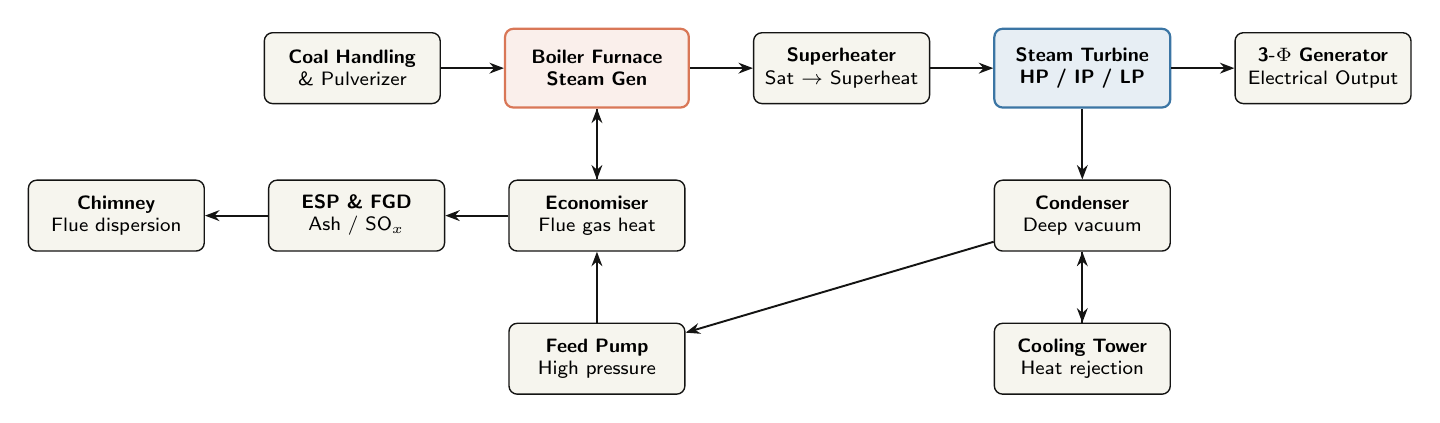
\begin{tikzpicture}[
  node distance=0.6cm and 0.8cm,
  block/.style={rectangle, draw=AnthDark, fill=AnthCardBG, rounded corners=3pt, line width=0.5pt, text width=2.0cm, align=center, minimum height=0.9cm, font=\scriptsize\sffamily},
  furnace/.style={rectangle, draw=AnthOrange, fill=AnthOrange!12, rounded corners=3pt, line width=0.8pt, text width=2.1cm, align=center, minimum height=1.0cm, font=\scriptsize\sffamily\bfseries},
  turb/.style={rectangle, draw=AnthBlue, fill=AnthBlue!12, rounded corners=3pt, line width=0.8pt, text width=2.0cm, align=center, minimum height=1.0cm, font=\scriptsize\sffamily\bfseries},
  arrow/.style={-{Stealth[scale=0.85]}, line width=0.7pt, color=AnthDark}
]
  \node[block] (coal) {\textbf{Coal Handling}\\ \& Pulverizer};
  \node[furnace, right=of coal] (boil) {\textbf{Boiler Furnace}\\ Steam Gen};
  \node[block, right=of boil] (sh) {\textbf{Superheater}\\ Sat $\to$ Superheat};
  \node[turb, right=of sh] (turb) {\textbf{Steam Turbine}\\ HP / IP / LP};
  \node[block, right=of turb] (gen) {\textbf{3-$\Phi$ Generator}\\ Electrical Output};

  \node[block, below=0.9cm of boil] (eco) {\textbf{Economiser}\\ Flue gas heat};
  \node[block, below=0.9cm of eco] (pump) {\textbf{Feed Pump}\\ High pressure};
  \node[block, below=0.9cm of turb] (cond) {\textbf{Condenser}\\ Deep vacuum};
  \node[block, below=0.9cm of cond] (ct) {\textbf{Cooling Tower}\\ Heat rejection};
  \node[block, left=of eco] (esp) {\textbf{ESP \& FGD}\\ Ash / $\text{SO}_x$};
  \node[block, left=of esp] (stack) {\textbf{Chimney}\\ Flue dispersion};

  \draw[arrow] (coal) -- (boil);
  \draw[arrow] (boil) -- (sh);
  \draw[arrow] (sh) -- (turb);
  \draw[arrow] (turb) -- (gen);
  \draw[arrow] (turb) -- (cond);
  \draw[arrow] (cond) -- (pump);
  \draw[arrow] (pump) -- (eco);
  \draw[arrow] (eco) -- (boil);
  \draw[arrow] (cond) -- (ct);
  \draw[arrow] (ct) -- (cond);
  \draw[arrow] (boil) -- (eco);
  \draw[arrow] (eco) -- (esp);
  \draw[arrow] (esp) -- (stack);
\end{tikzpicture}%
}
\end{center}

\concept{Major Sub-systems and Auxiliary Functions}
\begin{itemize}
  \item \textbf{Boiler \& Superheater:} Pulverized coal combustion evaporates water. Saturated steam is superheated to $540-600^\circ\text{C}$ to prevent moisture condensation and blade erosion inside the low-pressure turbine stages.
  \item \textbf{Economiser \& Air Preheater (APH):} Recover heat from exiting flue gas. The economiser preheats boiler feedwater, and the APH warms combustion air, increasing boiler efficiency by $5-10\%$.
  \item \textbf{Condenser:} Cools exhaust steam back to liquid water while maintaining a \textbf{high vacuum} ($0.05-0.08\,\text{bar}$ absolute), maximizing enthalpy drop and thermal efficiency.
  \item \textbf{Cooling Tower:} Dissipates heat from circulating condenser water. The white plume seen leaving cooling towers is \textbf{pure condensed water vapor}, not smoke.
  \item \textbf{Electrostatic Precipitator (ESP):} Applies high-voltage DC electric fields ($40-60\,\text{kV}$) to capture over $99.5\%$ of particulate fly ash before flue gas enters the stack.
  \item \textbf{Centrifugal Governor Valves:} Regulate steam mass flow into the high-pressure turbine to maintain constant synchronous speed ($3000\,\text{RPM}$ for 50 Hz, 2-pole) under changing electrical loads.
\end{itemize}

\concept{Fuels Utilized in Thermal Stations}
\begin{itemize}
  \item \textbf{Coal:} Mainstay for large baseload plants (Anthracite, Bituminous, Lignite).
  \item \textbf{Natural Gas:} Clean-burning methane fuel with lower carbon emissions per kWh.
  \item \textbf{Naphtha:} Liquid hydrocarbon mixture derived from crude refining. Used in plants such as \emph{NTPC Rajiv Gandhi CCPP (Kayamkulam, Kerala, 359 MW)}, which ran on naphtha before switching to pipeline natural gas via the Kochi--Mangaluru pipeline.
  \item \textbf{Low Sulphur Heavy Stock (LSHS) / Diesel:} Heavy residual fuel used for normal operation at \emph{Brahmapuram Diesel Power Plant (106.6 MW, Kochi)} and \emph{Kozhikode (Nallalam) Diesel Power Project (128 MW)}, which use diesel for starting and LSHS during normal operation.
  \item \textbf{Biomass:} Agricultural residues and wood pellets co-fired with coal to lower net carbon intensity.
\end{itemize}

\begin{Tip}[Thermal Engineering Benchmarks \& USC Technology]
\begin{itemize}
  \item Modern steam turbines operate at temperatures of \textbf{$540-600^\circ\text{C}$} and pressures exceeding \textbf{$25\,\text{MPa}$}.
  \item A single $1000\,\text{MW}$ thermal station can supply electricity to approximately \textbf{$700,000-1,000,000$ homes}.
  \item \textbf{Ultra-Supercritical (USC)} plants operate above the critical point of water ($22.064\,\text{MPa}$, $373.95^\circ\text{C}$), reaching efficiencies of \textbf{up to 47\%} and cutting emissions per MWh by $15-20\%$.
  \item \textbf{Prominent Thermal Plants:} \emph{Vindhyachal Super Thermal Power Station (Madhya Pradesh, 4,760 MW)} — India's largest thermal plant; \emph{Taichung Power Plant (Taiwan, 5,500 MW)} — one of the world's largest coal stations.
\end{itemize}
\end{Tip}

\begin{Note}[Advantages \& Disadvantages of Thermal Power]
\textbf{Advantages:} Highly reliable, continuous 24/7 baseload supply; lower upfront capital cost per MW and shorter gestation time than nuclear/hydro; flexible siting near coal mines (pithead) or load centers.\\
\textbf{Disadvantages:} Heavy greenhouse gas emissions ($\text{CO}_2$) and air pollutants ($\text{SO}_2, \text{NO}_x$, PM2.5); depletes fossil fuel reserves; requires substantial cooling water; creates fly ash disposal challenges.
\end{Note}

\concept{Environmental \& Ethical Considerations}
\begin{itemize}
  \item \textbf{Environmental:} Major contributor to climate change ($\text{CO}_2$); acid rain ($\text{SO}_2$); ground-level smog ($\text{NO}_x$); heavy metals (arsenic, lead, mercury) in fly ash ponds; thermal water discharge pollution.
  \item \textbf{Ethical:} Balancing affordable energy access against chronic public health issues in neighboring communities; ensuring a \textbf{Just Transition} for coal-dependent workforces as economies decarbonize.
\end{itemize}

%% ─────────────────────────────────────────────────────────────────────────────
\subsection{Nuclear Power Plants}

\concept{Working Principle \& Nuclear Fission Physics}
Nuclear power plants release the binding energy of atomic nuclei via controlled nuclear fission. When a fissile \textbf{Uranium-235 ($^{235}\text{U}$)} nucleus absorbs a thermal neutron, it splits into lighter fission fragments, releasing 2 to 3 fast neutrons and approximately $200\,\text{MeV}$ of energy per event.

\begin{Def}[Nuclear Fission Reaction Formula]
\begin{equation}
  {}^{235}_{\phantom{0}92}\text{U} + {}^1_0\text{n} \longrightarrow {}^{141}_{\phantom{0}56}\text{Ba} + {}^{92}_{36}\text{Kr} + 3\,{}^1_0\text{n} + \Delta E \quad (\approx 200\,\text{MeV})
\end{equation}
The mass defect $\Delta m$ is converted into thermal energy via $\Delta E = \Delta m \cdot c^2$. For sustained power, the effective multiplication factor is maintained at criticality ($k_{\text{eff}} = 1$).
\end{Def}

\concept{Energy Conversion Chain in Nuclear Plants}
\begin{align*}
  \text{Nuclear Binding Energy} &\xrightarrow{\text{Core Fission}} \text{Thermal Energy} \\
  &\xrightarrow{\text{Steam Turbine}} \text{Mechanical Energy} \xrightarrow{\text{Generator}} \text{Electrical Energy}
\end{align*}

\concept{Block Schematic of a Pressurized Water Reactor (PWR)}

\begin{center}
\resizebox{0.92\textwidth}{!}{%
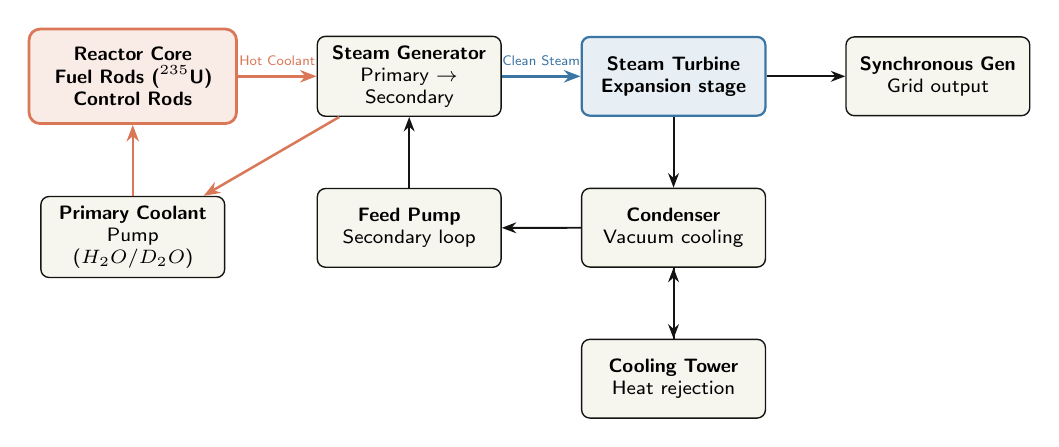
\begin{tikzpicture}[
  node distance=0.8cm and 1.0cm,
  core/.style={rectangle, draw=AnthOrange, fill=AnthOrange!15, rounded corners=4pt, line width=1.0pt, text width=2.4cm, align=center, minimum height=1.2cm, font=\scriptsize\sffamily\bfseries},
  block/.style={rectangle, draw=AnthDark, fill=AnthCardBG, rounded corners=3pt, line width=0.5pt, text width=2.1cm, align=center, minimum height=1.0cm, font=\scriptsize\sffamily},
  turb/.style={rectangle, draw=AnthBlue, fill=AnthBlue!12, rounded corners=3pt, line width=0.8pt, text width=2.1cm, align=center, minimum height=1.0cm, font=\scriptsize\sffamily\bfseries},
  arrow/.style={-{Stealth[scale=0.85]}, line width=0.7pt, color=AnthDark}
]
  \node[core] (core) {\textbf{Reactor Core}\\ Fuel Rods ($^{235}\text{U}$)\\ Control Rods};
  \node[block, right=of core] (sg) {\textbf{Steam Generator}\\ Primary $\to$ Secondary};
  \node[turb, right=of sg] (turb) {\textbf{Steam Turbine}\\ Expansion stage};
  \node[block, right=of turb] (gen) {\textbf{Synchronous Gen}\\ Grid output};

  \node[block, below=0.9cm of core] (pump1) {\textbf{Primary Coolant}\\ Pump ($H_2O / D_2O$)};
  \node[block, below=0.9cm of turb] (cond) {\textbf{Condenser}\\ Vacuum cooling};
  \node[block, below=0.9cm of sg] (pump2) {\textbf{Feed Pump}\\ Secondary loop};
  \node[block, below=0.9cm of cond] (ct) {\textbf{Cooling Tower}\\ Heat rejection};

  \draw[arrow, color=AnthOrange, line width=0.9pt] (core) -- node[above, font=\tiny\sffamily]{Hot Coolant} (sg);
  \draw[arrow, color=AnthOrange, line width=0.9pt] (sg) -- (pump1);
  \draw[arrow, color=AnthOrange, line width=0.9pt] (pump1) -- (core);

  \draw[arrow, color=AnthBlue, line width=0.9pt] (sg) -- node[above, font=\tiny\sffamily]{Clean Steam} (turb);
  \draw[arrow] (turb) -- (gen);
  \draw[arrow] (turb) -- (cond);
  \draw[arrow] (cond) -- (pump2);
  \draw[arrow] (pump2) -- (sg);
  \draw[arrow] (cond) -- (ct);
  \draw[arrow] (ct) -- (cond);
\end{tikzpicture}%
}
\end{center}

\concept{Major Reactor Components}
\begin{enumerate}
  \item \textbf{Fuel Rods:} Zircaloy tubes enclosing enriched ceramic $\text{UO}_2$ pellets ($3-5\%\ {}^{235}\text{U}$).
  \item \textbf{Control Rods:} Neutron-absorbing materials (Boron Carbide, Cadmium, Hafnium) that regulate fission rate or trigger instant emergency shutdown (\textbf{SCRAM}).
  \item \textbf{Moderator:} Slows fast fission neutrons ($\sim 2\,\text{MeV}$) to thermal energies ($\sim 0.025\,\text{eV}$) through elastic scattering ($H_2O, D_2O$, graphite).
  \item \textbf{Coolant:} Circulates through the core under high pressure ($15-16\,\text{MPa}$ in PWR) to transport fission heat without boiling.
  \item \textbf{Steam Generator:} Heat exchanger that isolates the radioactive primary loop from the non-radioactive secondary steam loop.
  \item \textbf{Containment Structure:} A massive prestressed concrete and steel dome ($1-2\,\text{m}$ thick) designed to contain radioactive releases during severe accidents.
\end{enumerate}

\begin{Tip}[Fuel Energy Density \& Submarine Endurance]
A single uranium fuel pellet ($\approx 7\,\text{g}$) produces energy equivalent to \textbf{nearly 1 metric tonne of coal}, $560\,\text{litres}$ of oil, or $480\,\text{m}^3$ of gas. An individual's entire lifetime electricity fuel requirement fits in a standard \textbf{330 mL beverage can}. Furthermore, nuclear submarines can stay submerged for months without refueling because a single reactor operates for years on one fuel load.
\end{Tip}

\concept{Prominent Stations \& Nuclear Safety Case Studies}
\begin{itemize}
  \item \textbf{Kudankulam Nuclear Power Plant (Tamil Nadu):} India's largest nuclear plant ($2 \times 1000\,\text{MW}$ VVER-1000 PWRs, expanding to $6,000\,\text{MW}$).
  \item \textbf{Kashiwazaki-Kariwa (Japan):} World's largest nuclear facility by installed capacity ($7,965\,\text{MW}$ spanning over $4.2\,\text{km}^2$, equal to 600 football fields).
  \item \textbf{Chernobyl Disaster (April 26, 1986, Ukraine/USSR):} Unauthorized safety test on an RBMK reactor with a positive void coefficient and flawed graphite-tipped control rods caused runaway prompt supercriticality, steam explosions, and destruction of the reactor building. Over 100,000 people were evacuated, leaving a $30\,\text{km}$ permanent exclusion zone. \emph{Lesson: Safe reactor design, proper training, strict procedures, and elimination of positive reactivity feedback.}
  \item \textbf{Fukushima Daiichi Disaster (March 11, 2011, Japan):} A magnitude 9.0 earthquake and 14m tsunami overtopped the 5.7m seawall, submerging emergency diesel generators and causing complete \textbf{Station Blackout (SBO)}. Loss of cooling caused core meltdowns and hydrogen explosions across three units ($150,000$ evacuated). \emph{Lesson: Plants must withstand extreme natural disasters, retain flood-proof power diversity, and deploy passive cooling systems.}
\end{itemize}

\begin{Note}[Advantages \& Disadvantages of Nuclear Power]
\textbf{Advantages:} Extremely high fuel energy density; near-zero operational greenhouse emissions; high capacity factors ($>90\%$); long plant operating life ($40-60+\,\text{years}$).\\
\textbf{Disadvantages:} Very high capital cost and lengthy licensing; long-lived High-Level Waste (HLW) management; public risk perception; complex decommissioning.
\end{Note}

%% ─────────────────────────────────────────────────────────────────────────────
\subsection{Choosing the Right Power Generation Method}

\begin{Note}[Generation Selection Matrix]
\begin{itemize}
  \item \textbf{Thermal Power Plants:} Best for reliable continuous base-load electricity where coal or gas is readily available.
  \item \textbf{Nuclear Power Plants:} Best for large-scale, low-carbon electricity generation with steady baseload output.
  \item \textbf{Hydroelectric Power Plants:} Best for mountainous regions with abundant rivers, excellent for peak-load and frequency support.
  \item \textbf{Solar Power Plants:} Best for high solar irradiance regions and distributed rooftop electricity generation.
  \item \textbf{Wind Power Plants:} Best for coastal areas, mountain passes, and open plains with strong, consistent wind flows.
\end{itemize}
\end{Note}

%% ─────────────────────────────────────────────────────────────────────────────
\clearpage
\section{Variable Renewable Energy Systems}
%% ─────────────────────────────────────────────────────────────────────────────

\syllabusitem{Solar and wind -- (block schematic details, environmental factors, regulations, advantages, disadvantages)}

\subsection{Solar Energy Systems}

Solar energy is captured via two primary routes: \textbf{Solar Photovoltaics (PV)} and \textbf{Solar Thermal (Concentrated Solar Power - CSP)}.

\concept{1. Solar Photovoltaic (PV) Generation}
Solar PV systems convert sunlight directly into DC electricity via the solid-state \textbf{photovoltaic effect} in semiconductor p-n junctions.

\begin{Def}[Photovoltaic Effect]
Incident photons with energy $h\nu \ge E_g$ create electron-hole pairs in the depletion region. The internal electric field sweeps electrons to the n-side and holes to the p-side, producing a DC voltage ($0.5-0.7\,\text{V}$ per silicon cell).
\end{Def}

\begin{center}
\resizebox{0.92\textwidth}{!}{%
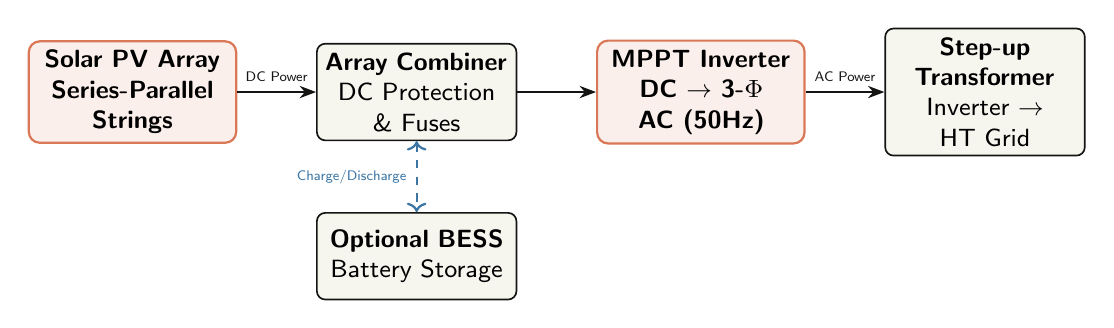
\begin{tikzpicture}[
  node distance=0.7cm and 1.0cm,
  block/.style={rectangle, draw=AnthDark, fill=AnthCardBG, rounded corners=3pt, line width=0.6pt, text width=2.3cm, align=center, minimum height=1.1cm, font=\small\sffamily},
  majorblock/.style={rectangle, draw=AnthOrange, fill=AnthOrange!12, rounded corners=4pt, line width=0.8pt, text width=2.4cm, align=center, minimum height=1.1cm, font=\small\sffamily\bfseries},
  arrow/.style={-{Stealth[scale=0.9]}, line width=0.8pt, color=AnthDark}
]
  \node[majorblock] (pv) {\textbf{Solar PV Array}\\ Series-Parallel Strings};
  \node[block, right=of pv] (combiner) {\textbf{Array Combiner}\\ DC Protection \& Fuses};
  \node[majorblock, right=of combiner] (inv) {\textbf{MPPT Inverter}\\ DC $\to$ 3-$\Phi$ AC (50Hz)};
  \node[block, right=of inv] (trans) {\textbf{Step-up Transformer}\\ Inverter $\to$ HT Grid};
  \node[block, below=0.9cm of combiner] (bess) {\textbf{Optional BESS}\\ Battery Storage};

  \draw[arrow] (pv) -- node[above, font=\tiny\sffamily]{DC Power} (combiner);
  \draw[arrow] (combiner) -- (inv);
  \draw[arrow] (inv) -- node[above, font=\tiny\sffamily]{AC Power} (trans);
  \draw[arrow, <->, dashed, color=AnthBlue] (combiner) -- node[left, font=\tiny\sffamily]{Charge/Discharge} (bess);
\end{tikzpicture}%
}
\end{center}

\begin{itemize}
  \item \textbf{PV Modules \& Tracking:} Cells connected in series/parallel. Trackers (single/dual-axis) follow the sun to increase generation by $15-25\%$.
  \item \textbf{MPPT Inverter:} Converts DC to 3-phase AC while tracking maximum power points across changing solar irradiance.
  \item \textbf{Floating Solar PV (FPV):} Panels installed on water bodies (e.g., \emph{NTPC Harippad / Kayamkulam 92 MW Floating Solar Project}), saving land, reducing water evaporation, and boosting module efficiency by $5-10\%$ through natural water cooling.
  \item \textbf{Famous Solar Parks:} \emph{Bhadla Solar Park (Rajasthan, 2,245 MW)} — situated in the Thar Desert where ambient temperatures exceed $45^\circ\text{C}$; \emph{Golmud Solar Park (Qinghai, China, >2,800 MW)} — massive high-altitude solar array visible from space.
\end{itemize}

\concept{2. Solar Thermal (Concentrated Solar Power - CSP)}
Uses mirrors (parabolic troughs or central towers) to focus solar irradiance onto a receiver, heating molten salt ($400-600^\circ\text{C}$) to drive a steam Rankine turbine. \textbf{Key Advantage:} Stored thermal energy enables continuous dispatch \textbf{for 6 to 16 hours after sunset} (e.g., \emph{Noor Ouarzazate, Morocco, 580 MW}).

\begin{Note}[Comparison: Solar PV vs. Solar Thermal (CSP)]
\begin{center}
\small
\begin{tabularx}{\linewidth}{L{3.0cm} X X}
  \rowcolor{AnthDark}
  \color{white}\textbf{Feature} & \color{white}\textbf{Solar Photovoltaic (PV)} & \color{white}\textbf{Solar Thermal (CSP)} \\
  \rowcolor{AnthCardBG} \textbf{Conversion} & Direct: Photons $\to$ DC Electricity & Thermodynamic: Photons $\to$ Heat $\to$ Steam $\to$ AC \\
  \textbf{Storage} & Electrochemical batteries (BESS) & Molten salt thermal storage (TES) \\
  \rowcolor{AnthCardBG} \textbf{Water Usage} & Minimal (cleaning only) & High (condenser cooling) \\
  \textbf{Dispatchability} & Intermittent without BESS & Dispatchable into night peak via TES \\
\end{tabularx}
\end{center}
\end{Note}

%% ─────────────────────────────────────────────────────────────────────────────
\subsection{Wind Energy Systems}

\concept{Working Principle \& Aerodynamics}
Wind turbines convert atmospheric kinetic energy into mechanical shaft power via aerodynamic lift on aerofoil blades:
\begin{equation}
  P_{\text{wind}} = \frac{1}{2} \rho A v^3 \quad \text{[Watts]}, \qquad P_{\text{mech}} = \frac{1}{2} \rho A v^3 C_p(\lambda, \beta)
\end{equation}
where maximum theoretical aerodynamic efficiency is governed by the \textbf{Betz Limit} ($C_{p,\text{max}} = 16/27 \approx 59.3\%$).

\begin{center}
\resizebox{0.92\textwidth}{!}{%
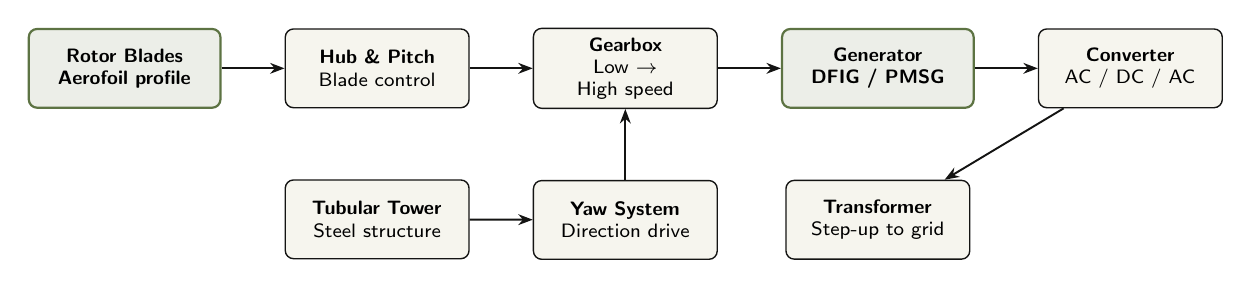
\begin{tikzpicture}[
  node distance=0.6cm and 0.8cm,
  block/.style={rectangle, draw=AnthDark, fill=AnthCardBG, rounded corners=3pt, line width=0.5pt, text width=2.1cm, align=center, minimum height=1.0cm, font=\scriptsize\sffamily},
  majorblock/.style={rectangle, draw=AnthGreen, fill=AnthGreen!12, rounded corners=3pt, line width=0.8pt, text width=2.2cm, align=center, minimum height=1.0cm, font=\scriptsize\sffamily\bfseries},
  arrow/.style={-{Stealth[scale=0.85]}, line width=0.7pt, color=AnthDark}
]
  \node[majorblock] (blades) {\textbf{Rotor Blades}\\ Aerofoil profile};
  \node[block, right=of blades] (hub) {\textbf{Hub \& Pitch}\\ Blade control};
  \node[block, right=of hub] (gear) {\textbf{Gearbox}\\ Low $\to$ High speed};
  \node[majorblock, right=of gear] (gen) {\textbf{Generator}\\ DFIG / PMSG};
  \node[block, right=of gen] (conv) {\textbf{Converter}\\ AC / DC / AC};

  \node[block, below=0.9cm of gen] (trans) {\textbf{Transformer}\\ Step-up to grid};
  \node[block, below=0.9cm of gear] (yaw) {\textbf{Yaw System}\\ Direction drive};
  \node[block, below=0.9cm of hub] (tower) {\textbf{Tubular Tower}\\ Steel structure};

  \draw[arrow] (blades) -- (hub);
  \draw[arrow] (hub) -- (gear);
  \draw[arrow] (gear) -- (gen);
  \draw[arrow] (gen) -- (conv);
  \draw[arrow] (conv) -- (trans);
  \draw[arrow] (yaw) -- (gear);
  \draw[arrow] (tower) -- (yaw);
\end{tikzpicture}%
}
\end{center}

\begin{itemize}
  \item \textbf{Pitch Control:} Adjusts blade angle along its axis to optimize aerodynamic lift or feather blades in high winds.
  \item \textbf{Gearbox \& Generator:} Steps up low rotor speed ($10-20\,\text{RPM}$) to generator speed ($1500\,\text{RPM}$); uses DFIG or direct-drive PMSG.
  \item \textbf{Yaw Mechanism:} Keeps the nacelle facing directly into the wind based on wind-vane signals.
  \item \textbf{Onshore vs Offshore:} Offshore captures stronger, steadier marine winds yielding \textbf{capacity factors $>50\%$}.
  \item \textbf{Notable Projects:} \emph{Muppandal Wind Farm (Tamil Nadu, ~1500 MW)}, capturing Western Ghats mountain pass winds; \emph{Gansu Wind Farm (China, 20,000 MW planned)}.
  \item \textbf{Environmental Impacts:} Low-frequency acoustic noise, shadow flicker, landscape aesthetics, and bird/bat collision risks.
\end{itemize}

%% ─────────────────────────────────────────────────────────────────────────────
\subsection{Renewable Energy Policies, Regulations \& Future Horizons}

\begin{enumerate}
  \item \textbf{National Solar Mission (JNNSM 2010, India):} Catalyzed competitive bidding, driving solar tariffs from over $\text{Rs. } 12/\text{kWh}$ (2010) down below $\text{Rs. } 2.50/\text{kWh}$.
  \item \textbf{Renewable Purchase Obligation (RPO):} Legal mandate under the Electricity Act 2003 requiring utilities and open-access consumers to purchase a designated percentage of renewable power (Solar, Non-solar, HPO).
  \item \textbf{PM Surya Ghar: Muft Bijli Yojana (2024):} Subsidies for 1 crore households for up to $3\,\text{kW}$ rooftop solar, providing up to 300 free units/month.
  \item \textbf{National Wind-Solar Hybrid Policy (2018):} Co-locates wind and solar at shared evacuation substations to optimize transmission utilization.
  \item \textbf{India's 500 GW Target (2030):} National commitment to install $500\,\text{GW}$ non-fossil capacity by 2030.
  \item \textbf{Global Policies:} Renewable Portfolio Standards (RPS), Feed-in Tariffs (FiT), Reverse Auctions, Net/Gross Metering, Carbon Pricing / Emissions Trading Systems (ETS).
  \item \textbf{Supply Chain Ethics \& Agrivoltaics:} Managing environmental footprints from mining \textbf{lithium, cobalt, and rare earth elements} in fragile ecosystems; adopting \textbf{agrivoltaics} to allow dual-use farming beneath solar panels.
  \item \textbf{Future Horizons:} \textbf{Green Hydrogen} via electrolysis for seasonal multi-day storage; \textbf{Nuclear Fusion} (ITER project, 2040s horizon) for baseload carbon-free energy.
\end{enumerate}

%% ─────────────────────────────────────────────────────────────────────────────
\clearpage
\section{Energy Storage Systems (ESS) as Alternative Sources}
%% ─────────────────────────────────────────────────────────────────────────────

\syllabusitem{Energy storage systems as alternative energy sources -- BESS, CESS, thermal SS}

\subsection{Need for Energy Storage in Modern Grids}
Energy storage addresses renewable intermittency, mitigates steep evening ramping (\emph{the Duck Curve}), provides synthetic inertia, captures curtailed energy, and supports frequency regulation.

\begin{center}
\resizebox{0.88\textwidth}{!}{%
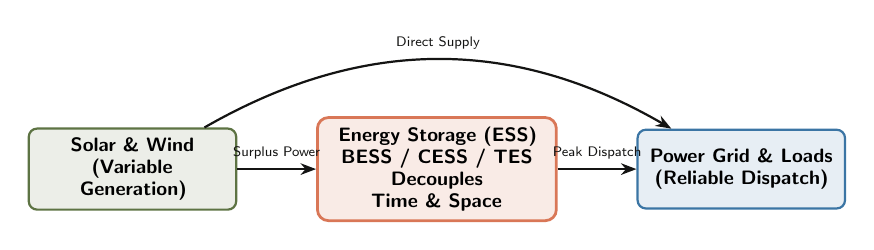
\begin{tikzpicture}[
  node distance=0.8cm and 1.0cm,
  source/.style={rectangle, draw=AnthGreen, fill=AnthGreen!12, rounded corners=3pt, line width=0.8pt, text width=2.4cm, align=center, minimum height=1.0cm, font=\scriptsize\sffamily\bfseries},
  ess/.style={rectangle, draw=AnthOrange, fill=AnthOrange!15, rounded corners=4pt, line width=1.0pt, text width=2.8cm, align=center, minimum height=1.1cm, font=\scriptsize\sffamily\bfseries},
  grid/.style={rectangle, draw=AnthBlue, fill=AnthBlue!12, rounded corners=3pt, line width=0.8pt, text width=2.4cm, align=center, minimum height=1.0cm, font=\scriptsize\sffamily\bfseries},
  arrow/.style={-{Stealth[scale=0.85]}, line width=0.8pt, color=AnthDark}
]
  \node[source] (solar) {Solar \& Wind\\ (Variable Generation)};
  \node[ess, right=1.0cm of solar] (ess) {\textbf{Energy Storage (ESS)}\\ BESS / CESS / TES\\ \emph{Decouples Time \& Space}};
  \node[grid, right=1.0cm of ess] (grid) {Power Grid \& Loads\\ (Reliable Dispatch)};

  \draw[arrow] (solar) -- node[above, font=\tiny\sffamily]{Surplus Power} (ess);
  \draw[arrow] (ess) -- node[above, font=\tiny\sffamily]{Peak Dispatch} (grid);
  \draw[arrow] (solar) to[bend left=30] node[above, font=\tiny\sffamily]{Direct Supply} (grid);
\end{tikzpicture}%
}
\end{center}

\subsection{Battery Energy Storage Systems (BESS)}
\begin{itemize}
  \item \textbf{Chemistries:} Lithium Iron Phosphate ($\text{LiFePO}_4$ / LFP) for thermal safety and cycle life; Nickel Manganese Cobalt (NMC) for energy density; Flow Batteries (Vanadium Redox) for long-duration bulk storage; emerging Solid-State batteries.
  \item \textbf{Performance:} Fast sub-second response ($<100\,\text{ms}$) for frequency regulation; high round-trip efficiency ($85-95\%$); $1-4\,\text{hour}$ discharge duration; requires Battery Management Systems (BMS) with liquid cooling to prevent thermal runaway.
  \item \textbf{Benchmark:} \emph{Hornsdale Power Reserve (Tesla Megapack, 150 MW / 193.5 MWh, South Australia)}.
\end{itemize}

\subsection{Compressed Air Energy Storage (CESS / CAES)}
\begin{itemize}
  \item \textbf{Mechanism:} Off-peak power compresses air ($40-80\,\text{bar}$) into underground sealed salt caverns, depleted aquifers, or rock mines; peak demand releases air through preheaters and expander turbines driving generators.
  \item \textbf{Features:} Multi-hour to multi-day bulk capacity (hundreds of MWh); long life ($>30\,\text{years}$); efficiency $40-70\%$; tied to geological formations.
\end{itemize}

\subsection{Thermal Energy Storage (TES / Thermal SS)}
\begin{itemize}
  \item \textbf{Media:} Molten salts ($290-565^\circ\text{C}$), pressurized hot water, Phase Change Materials (PCMs), chilled water/ice for HVAC peak shaving.
  \item \textbf{Applications:} CSP evening generation, industrial process heat, and district heating/cooling.
\end{itemize}

\subsection{Comprehensive Comparison Matrix of Storage Technologies}

\begin{center}
\small
\begin{tabularx}{\textwidth}{L{2.5cm} C{2.0cm} C{2.0cm} C{2.2cm} X}
  \rowcolor{AnthDark}
  \color{white}\textbf{Technology} & \color{white}\textbf{Efficiency} & \color{white}\textbf{Response} & \color{white}\textbf{Duration} & \color{white}\textbf{Primary Grid Services} \\
  \rowcolor{AnthCardBG} \textbf{BESS (Li-ion)} & $85-95\%$ & Milliseconds & 15 min -- 4 hrs & Frequency regulation, synthetic inertia, fast peak shaving \\
  \textbf{CESS (CAES)} & $40-70\%$ & 5 -- 15 min & 4 -- 24+ hrs & Bulk energy shifting, seasonal balancing \\
  \rowcolor{AnthCardBG} \textbf{Thermal SS (TES)} & $50-80\%$ & Minutes & 4 -- 16 hrs & CSP night dispatch, HVAC load shifting \\
  \textbf{Pumped Hydro (PSH)} & $70-85\%$ & 1 -- 3 min & 6 -- 20+ hrs & Bulk baseload storage, black start \\
\end{tabularx}
\end{center}

%% ─────────────────────────────────────────────────────────────────────────────
\clearpage
\section{Load Curves, Station Economics \& Mathematical Formulations}
%% ─────────────────────────────────────────────────────────────────────────────

\syllabusitem{Load curve -- Load duration curve, Load factor, diversity factor, demand factor, Plant capacity factor, plant use factor - Numerical Problems.}

\subsection{Load Dynamics and Operational Challenges}

\concept{The Invisible Challenge: Why Power Cannot Wait}
Unlike gas or water, bulk electrical energy cannot be warehoused directly on transmission lines. Generation must match consumption instantaneously across shifting human behavior.

\concept{When Variables Collide}
\begin{itemize}
  \item \textbf{Equipment Wear:} Frequent load cycling induces thermal fatigue in turbine blades and boiler tubes, accelerating maintenance schedules.
  \item \textbf{Fuel Efficiency:} Thermal plants operated below rated capacity suffer a \textbf{$15-25\%$ part-load heat rate penalty}.
  \item \textbf{System Responsiveness:} Fast load changes demand unloaded spinning reserves, imposing an efficiency penalty across the fleet.
\end{itemize}

\concept{The Future of Load Management}
\begin{itemize}
  \item \textbf{Smart Grids:} Real-time bidirectional communication enabling automated \textbf{Demand-Side Management (DSM)} to flatten load curves.
  \item \textbf{AI-Driven Forecasting:} Machine learning models predict demand surges hours in advance using weather and historical data.
  \item \textbf{Dynamic Grid Intelligence:} Self-optimizing grid systems balancing cost, carbon emissions, and reliability.
\end{itemize}

%% ─────────────────────────────────────────────────────────────────────────────
\subsection{The Load Curve and Load Duration Curve}

\begin{Def}[Load Curve vs. Load Duration Curve]
\textbf{Load Curve:} Chronological plot of power demand (kW/MW) vs time (hours). Area under curve = Total Energy ($E$).\\
\textbf{Load Duration Curve (LDC):} Chronological load rearranged in \textbf{descending order of magnitude}.
\begin{equation}
  E = \int_{0}^{T} P(t)\,dt = \sum_{i=1}^{n} P_i \cdot \Delta t_i \quad [\text{kWh or MWh}], \qquad L_{\text{avg}} = \frac{E}{T} \quad [\text{kW or MW}]
\end{equation}
\end{Def}

\begin{center}
\resizebox{0.88\textwidth}{!}{%
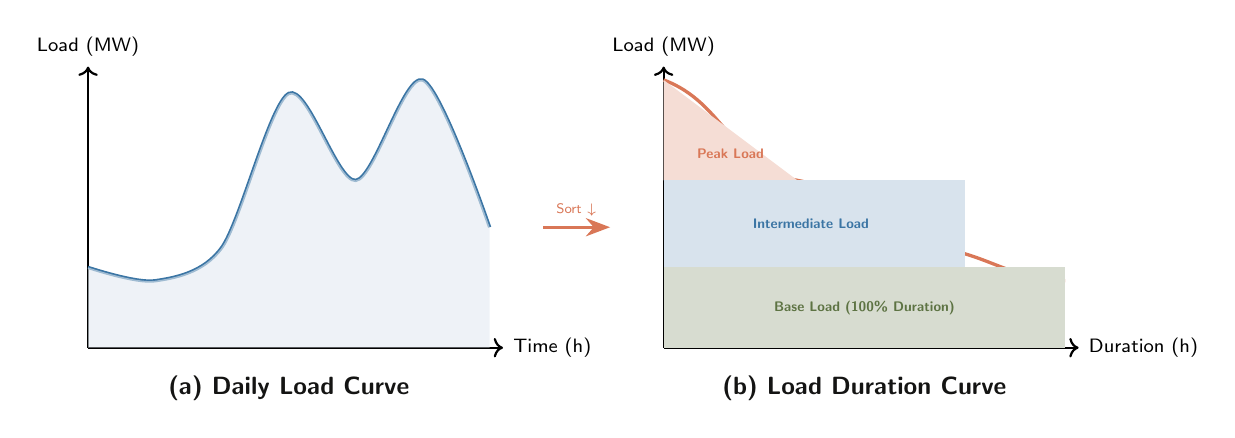
\begin{tikzpicture}[scale=0.85]
  %% Chronological Load Curve (Left)
  \begin{scope}[xshift=0cm]
    \draw[line width=0.8pt, ->] (0,0) -- (6.2,0) node[right, font=\scriptsize\sffamily]{Time (h)};
    \draw[line width=0.8pt, ->] (0,0) -- (0,4.2) node[above, font=\scriptsize\sffamily]{Load (MW)};
    \draw[color=AnthBlue, line width=1.2pt] plot[smooth] coordinates {
      (0,1.2) (1,1.0) (2,1.5) (3,3.8) (4,2.5) (5,4.0) (6,1.8)
    };
    \fill[AnthBlue!15, opacity=0.6] (0,0) -- plot[smooth] coordinates {
      (0,1.2) (1,1.0) (2,1.5) (3,3.8) (4,2.5) (5,4.0) (6,1.8)
    } -- (6,0) -- cycle;
    \node[font=\small\sffamily\bfseries, color=AnthDark] at (3, -0.6) {(a) Daily Load Curve};
  \end{scope}

  \draw[-{Stealth[scale=1.1]}, line width=1.1pt, color=AnthOrange] (6.8, 1.8) -- (7.8, 1.8) node[midway, above, font=\tiny\sffamily]{Sort $\downarrow$};

  %% Load Duration Curve (Right)
  \begin{scope}[xshift=8.6cm]
    \draw[line width=0.8pt, ->] (0,0) -- (6.2,0) node[right, font=\scriptsize\sffamily]{Duration (h)};
    \draw[line width=0.8pt, ->] (0,0) -- (0,4.2) node[above, font=\scriptsize\sffamily]{Load (MW)};
    
    \draw[color=AnthOrange, line width=1.2pt] (0,4.0) to[out=-20, in=170] (2.0,2.5) to[out=-10, in=175] (4.0,1.5) to[out=-5, in=180] (6.0,1.0);
    
    \fill[AnthOrange!25] (0,2.5) -- plot[domain=0:2.0] ({(\x)},{4.0 - 0.75*\x}) -- (2.0,2.5) -- cycle;
    \fill[AnthBlue!20] (0,1.2) rectangle (4.5,2.5);
    \fill[AnthGreen!25] (0,0) rectangle (6.0,1.2);

    \node[font=\tiny\sffamily\bfseries, color=AnthOrange] at (1.0, 2.9) {Peak Load};
    \node[font=\tiny\sffamily\bfseries, color=AnthBlue] at (2.2, 1.85) {Intermediate Load};
    \node[font=\tiny\sffamily\bfseries, color=AnthGreen] at (3.0, 0.6) {Base Load (100\% Duration)};

    \node[font=\small\sffamily\bfseries, color=AnthDark] at (3, -0.6) {(b) Load Duration Curve};
  \end{scope}
\end{tikzpicture}%
}
\end{center}

%% ─────────────────────────────────────────────────────────────────────────────
\subsection{Mathematical Definitions of Economic Factors}

\begin{enumerate}
  \item \textbf{Connected Load:} Continuous sum of continuous ratings of all connected appliances.
  \item \textbf{Maximum Demand ($MD$):} Greatest load drawn during a specified 15/30-minute interval.
  \item \textbf{Demand Factor ($DF$):}
    \begin{equation}
      DF = \frac{\text{Maximum Demand}}{\text{Connected Load}} \le 1
    \end{equation}
    \emph{Typical values: Domestic $0.4-0.6$, Commercial $0.5-0.8$, Industrial $0.7-0.95$.}
  \item \textbf{Load Factor ($LF$):}
    \begin{equation}
      LF = \frac{\text{Average Load}}{\text{Maximum Demand}} = \frac{\text{Energy Generated in time } T}{MD \times T} \le 1
    \end{equation}
  \item \textbf{Diversity Factor ($DivF$):}
    \begin{equation}
      DivF = \frac{\sum_{k=1}^{n} MD_k}{\text{Coincident System Maximum Demand}} \ge 1
    \end{equation}
  \item \textbf{Plant Capacity Factor ($PCF$):}
    \begin{equation}
      PCF = \frac{\text{Actual Energy Generated}}{\text{Installed Plant Capacity} \times T} = \frac{L_{\text{avg}}}{\text{Installed Capacity}} \le 1
    \end{equation}
    \begin{equation}
      \text{Reserve Capacity} = \text{Installed Plant Capacity} - \text{Maximum Demand}
    \end{equation}
    \begin{equation}
      PCF = LF \times \left(\frac{MD}{\text{Installed Capacity}}\right) = LF \times \text{Utilization Factor}
    \end{equation}
  \item \textbf{Plant Use Factor ($PUF$):}
    \begin{equation}
      PUF = \frac{\text{Actual Energy Generated}}{\text{Installed Capacity} \times T_{\text{operating}}} \ge PCF
    \end{equation}
  \item \textbf{Utilization Factor ($UF$):} $UF = \frac{\text{Maximum Demand}}{\text{Installed Capacity}} \le 1$.
\end{enumerate}

\begin{Tip}[The Power Engineer's Mandate]
A \textbf{1\% improvement in load factor} across a $1,000\,\text{MW}$ generation fleet represents millions of dollars in avoided capital and fuel expenditure annually.
\end{Tip}

%% ─────────────────────────────────────────────────────────────────────────────
\subsection{Fully Worked-Out Numerical Problems}

\begin{Problem}[Problem 1: Residential Distribution Feeder \& Capacity Sizing]
A housing township has 3 groups: Group A (50 homes, connected load $2,500\,\text{kW}$, $DF = 0.5$), Group B (30 shops, connected load $1,800\,\text{kW}$, $DF = 0.6$), Group C (20 community facilities, connected load $1,200\,\text{kW}$, $DF = 0.55$). Diversity factor = $1.40$. Find individual max demands, sum, system max demand, transformer rating, and capacity saving.
\end{Problem}

\begin{Solution}
\begin{enumerate}
  \item Individual Demands:
    $MD_A = 2500 \times 0.5 = 1,250\,\text{kW}$,
    $MD_B = 1800 \times 0.6 = 1,080\,\text{kW}$,
    $MD_C = 1200 \times 0.55 = 660\,\text{kW}$.
  \item Sum of Individual Peaks: $\sum MD_i = 1250 + 1080 + 660 = \mathbf{2,990\,\text{kW}}$.
  \item System Coincident Peak: $MD_{\text{system}} = \frac{2990}{1.40} = \mathbf{2,135.71\,\text{kW}} \approx \mathbf{2,136\,\text{kW}}$.
  \item Transformer Rating Required = \textbf{2,136 kW}.
  \item Capacity Saving: $\frac{5500 - 2135.71}{5500} \times 100\% = \mathbf{61.17\%}$.
\end{enumerate}
\end{Solution}

\begin{Problem}[Problem 2: Daily Step-Load Schedule Analysis]
A $100\,\text{MW}$ station has the daily schedule: $00-06\text{h}$ ($40\,\text{MW}$), $06-12\text{h}$ ($80\,\text{MW}$), $12-18\text{h}$ ($100\,\text{MW}$), $18-24\text{h}$ ($60\,\text{MW}$). Find daily energy, annual energy, average load, load factor, and plant capacity factor.
\end{Problem}

\begin{Solution}
\begin{enumerate}
  \item Daily Energy: $E_{\text{daily}} = (40\times 6) + (80\times 6) + (100\times 6) + (60\times 6) = 240 + 480 + 600 + 360 = \mathbf{1,680\,\text{MWh}}$.
  \item Annual Energy: $E_{\text{annual}} = 1680 \times 365 = \mathbf{613,200\,\text{MWh}}$.
  \item Average Load: $L_{\text{avg}} = \frac{1680}{24} = \mathbf{70\,\text{MW}}$.
  \item Load Factor: $LF = \frac{70}{100} = \mathbf{0.70} = \mathbf{70\%}$.
  \item Plant Capacity Factor: $PCF = \frac{70}{100} = \mathbf{70\%}$.
\end{enumerate}
\end{Solution}

\begin{Problem}[Problem 3: Comparative Economic Evaluation of Two Power Stations]
Plant A ($100\,\text{MW}$ cap, $80\,\text{MW}$ peak) and Plant B ($150\,\text{MW}$ cap, $100\,\text{MW}$ peak) each generate $500,000\,\text{MWh}$ annually. Compare average load, load factor, capacity factor, reserve capacity, and economics.
\end{Problem}

\begin{Solution}
\begin{enumerate}
  \item Average Load: $L_{\text{avg}} = \frac{500,000}{8760} = \mathbf{57.08\,\text{MW}}$ for both plants.
  \item Load Factor: $LF_A = \frac{57.08}{80} = \mathbf{71.35\%}$; $LF_B = \frac{57.08}{100} = \mathbf{57.08\%}$.
  \item Capacity Factor: $PCF_A = \frac{57.08}{100} = \mathbf{57.08\%}$; $PCF_B = \frac{57.08}{150} = \mathbf{38.05\%}$.
  \item Reserve: $\text{Res}_A = 100 - 80 = \mathbf{20\,\text{MW}}$; $\text{Res}_B = 150 - 100 = \mathbf{50\,\text{MW}}$.
  \item \textbf{Economic Verdict:} Plant A generates the same energy from lower capital capacity, achieving much higher load factor and lower unit generation cost.
\end{enumerate}
\end{Solution}

\begin{Problem}[Problem 4: Load Factor Calculation]
Maximum demand = $80\,\text{MW}$, Daily energy = $1200\,\text{MWh}$. Find Average Load and Load Factor.
\end{Problem}

\begin{Solution}
$L_{\text{avg}} = \frac{1200}{24} = \mathbf{50\,\text{MW}}$, \qquad $LF = \frac{50}{80} = \mathbf{0.625} = \mathbf{62.5\%}$.
\end{Solution}

\begin{Problem}[Problem 5: Demand Factor Calculation]
Connected Load = $500\,\text{kW}$, Maximum Demand = $350\,\text{kW}$. Find Demand Factor.
\end{Problem}

\begin{Solution}
$DF = \frac{350}{500} = \mathbf{0.70} = \mathbf{70\%}$.
\end{Solution}

\begin{Problem}[Problem 6: Diversity Factor Calculation]
Consumer demands: $40, 60, 80, 100\,\text{kW}$. System coincident peak = $200\,\text{kW}$. Find Diversity Factor.
\end{Problem}

\begin{Solution}
$\sum MD_i = 40+60+80+100 = 280\,\text{kW}$, \qquad $DivF = \frac{280}{200} = \mathbf{1.40}$.
\end{Solution}

\begin{Problem}[Problem 7: Plant Capacity Factor Calculation]
Capacity = $100\,\text{MW}$, Daily Energy = $1440\,\text{MWh}$. Find Plant Capacity Factor.
\end{Problem}

\begin{Solution}
$PCF = \frac{1440}{100 \times 24} = \frac{1440}{2400} = \mathbf{0.60} = \mathbf{60\%}$.
\end{Solution}

\begin{Problem}[Problem 8: Plant Use Factor with Operating Outages]
Capacity = $120\,\text{MW}$, Operating time = $16\,\text{hours/day}$, Daily Energy = $1440\,\text{MWh}$. Find Plant Use Factor and Capacity Factor.
\end{Problem}

\begin{Solution}
$PUF = \frac{1440}{120 \times 16} = \frac{1440}{1920} = \mathbf{0.75} = \mathbf{75\%}$, \qquad $PCF = \frac{1440}{120 \times 24} = \frac{1440}{2880} = \mathbf{50\%}$.
\end{Solution}

\begin{Problem}[Problem 9: Multi-Parameter Station Analysis]
Installed Capacity = $150\,\text{MW}$, Maximum Demand = $120\,\text{MW}$, Connected Load = $180\,\text{MW}$, Daily Energy = $2160\,\text{MWh}$. Determine: (a) $L_{\text{avg}}$, (b) $LF$, (c) $DF$, (d) $PCF$, (e) Reserve Capacity.
\end{Problem}

\begin{Solution}
\begin{enumerate}
  \item $L_{\text{avg}} = \frac{2160}{24} = \mathbf{90\,\text{MW}}$.
  \item $LF = \frac{90}{120} = \mathbf{0.75} = \mathbf{75\%}$.
  \item $DF = \frac{120}{180} = \mathbf{0.667} = \mathbf{66.7\%}$.
  \item $PCF = \frac{2160}{150 \times 24} = \mathbf{0.60} = \mathbf{60\%}$.
  \item $\text{Reserve} = 150 - 120 = \mathbf{30\,\text{MW}}$.
\end{enumerate}
\end{Solution}

\begin{Problem}[Problem 10: Complete Operational Analysis]
Capacity = $200\,\text{MW}$, Operating Hours = $18\,\text{h}$, Daily Energy = $2520\,\text{MWh}$, Connected Load = $240\,\text{MW}$, $MD = 180\,\text{MW}$. Determine $L_{\text{avg}}$, $LF$, $DF$, $PCF$, $PUF$, and $UF$.
\end{Problem}

\begin{Solution}
\begin{enumerate}
  \item $L_{\text{avg}} = \frac{2520}{24} = \mathbf{105\,\text{MW}}$.
  \item $LF = \frac{105}{180} = \mathbf{0.5833} = \mathbf{58.33\%}$.
  \item $DF = \frac{180}{240} = \mathbf{0.75} = \mathbf{75\%}$.
  \item $PCF = \frac{2520}{200 \times 24} = \frac{2520}{4800} = \mathbf{52.5\%}$.
  \item $PUF = \frac{2520}{200 \times 18} = \frac{2520}{3600} = \mathbf{70\%}$.
  \item $UF = \frac{180}{200} = \mathbf{0.90} = \mathbf{90\%}$.
\end{enumerate}
\end{Solution}

\begin{Problem}[Problem 11: Linear Load Duration Curve Integration]
An annual load duration curve slopes linearly from $120\,\text{MW}$ to $30\,\text{MW}$ over 8,760 hours. Find total energy, average load, load factor, and base/peak energy if a $40\,\text{MW}$ base plant is used.
\end{Problem}

\begin{Solution}
\begin{align*}
  E_{\text{total}} &= \left(\frac{120 + 30}{2}\right) \times 8760 = 75 \times 8760 = \mathbf{657,000\,\text{MWh}} \\
  L_{\text{avg}} &= \frac{657,000}{8760} = \mathbf{75\,\text{MW}}, \qquad LF = \frac{75}{120} = \mathbf{0.625} = \mathbf{62.5\%} \\
  E_{\text{base}} &= 40 \times 8760 = \mathbf{350,400\,\text{MWh}} \quad (53.33\%) \\
  E_{\text{peak}} &= 657,000 - 350,400 = \mathbf{306,600\,\text{MWh}} \quad (46.67\%)
\end{align*}
\end{Solution}

\begin{Problem}[Problem 12: Generation Tariff Economics]
A $50\,\text{MW}$ station operates at annual load factor $60\%$. Capital cost = $\text{Rs. } 5\,\text{crore/MW}$, annual fixed charges = $12\%$, fuel/operating cost = $\text{Rs. } 2.20/\text{kWh}$. Calculate total annual cost and cost per kWh generated.
\end{Problem}

\begin{Solution}
\begin{align*}
  L_{\text{avg}} &= 50,000\,\text{kW} \times 0.60 = 30,000\,\text{kW} \\
  E_{\text{annual}} &= 30,000 \times 8760 = 262.8 \times 10^6\,\text{kWh} \\
  \text{Fixed Cost} &= 12\% \times (50 \times \text{Rs. } 5 \times 10^7) = \text{Rs. } 30 \times 10^7 = \text{Rs. } 300 \times 10^6 \\
  \text{Variable Cost} &= 262.8 \times 10^6 \times \text{Rs. } 2.20 = \text{Rs. } 578.16 \times 10^6 \\
  \text{Total Cost} &= \text{Rs. } 878.16 \times 10^6 \\
  \text{Cost per kWh} &= \frac{878.16 \times 10^6}{262.8 \times 10^6} = \mathbf{\text{Rs. } 3.34/\text{kWh}} \quad (\text{Fixed: Rs. 1.14}, \text{Variable: Rs. 2.20})
\end{align*}
\end{Solution}

%% ─────────────────────────────────────────────────────────────────────────────
\clearpage
\section{Quick Revision Sheet \& Model Examination Questions}
%% ─────────────────────────────────────────────────────────────────────────────

\subsection{Master Formula and Definition Summary Table}

\begin{center}
\small
\begin{tabularx}{\textwidth}{L{3.0cm} L{4.8cm} C{1.8cm} X}
  \rowcolor{AnthDark}
  \color{white}\textbf{Factor / Metric} & \color{white}\textbf{Formula} & \color{white}\textbf{Typical Value} & \color{white}\textbf{Physical Significance} \\
  \rowcolor{AnthCardBG} \textbf{Demand Factor ($DF$)} & $\frac{\text{Maximum Demand}}{\text{Connected Load}}$ & $\le 1$ ($0.4 - 0.8$) & Non-simultaneous load operation; sizes feeder rating \\
  \textbf{Load Factor ($LF$)} & $\frac{\text{Average Load}}{\text{Maximum Demand}} = \frac{\text{Energy}}{MD \times T}$ & $\le 1$ ($0.5 - 0.85$) & Steady plant utilization; higher $LF$ cuts unit generation cost \\
  \rowcolor{AnthCardBG} \textbf{Diversity Factor ($DivF$)} & $\frac{\sum \text{Individual Peaks}}{\text{System Peak Demand}}$ & $\ge 1$ ($1.2 - 1.6$) & Staggered consumer peaks; reduces required station size \\
  \textbf{Capacity Factor ($PCF$)} & $\frac{\text{Actual Energy}}{\text{Installed Capacity} \times T} = \frac{L_{\text{avg}}}{\text{Cap}}$ & $\le 1$ ($0.4 - 0.8$) & Capital asset utilization index \\
  \rowcolor{AnthCardBG} \textbf{Reserve Capacity} & $\text{Installed Capacity} - MD$ & $\ge 0\,\text{MW}$ & Safeguards against outages and peak surges \\
  \textbf{Plant Use Factor ($PUF$)} & $\frac{\text{Actual Energy}}{\text{Installed Capacity} \times T_{\text{op}}}$ & $\ge PCF$ & Operational efficiency during active run-time \\
  \rowcolor{AnthCardBG} \textbf{Utilization Factor ($UF$)} & $\frac{\text{Maximum Demand}}{\text{Installed Capacity}}$ & $\le 1$ ($0.7 - 0.95$) & Fraction of station capacity demanded at peak \\
\end{tabularx}
\end{center}

\subsection{Master Comparison Matrix of All Power Generation Sources}

\begin{center}
\scriptsize
\begin{tabularx}{\textwidth}{L{1.8cm} L{2.6cm} L{2.4cm} L{2.2cm} L{2.4cm} X}
  \rowcolor{AnthDark}
  \color{white}\textbf{Feature} & \color{white}\textbf{Hydroelectric} & \color{white}\textbf{Thermal (Coal)} & \color{white}\textbf{Nuclear} & \color{white}\textbf{Solar PV} & \color{white}\textbf{Wind Energy} \\
  \rowcolor{AnthCardBG} \textbf{Primary Source} & Gravitational potential & Chemical (coal/gas) & Nuclear fission ($^{235}\text{U}$) & Solar photons & Kinetic wind flow \\
  \textbf{Cycle / Mode} & Hydraulic turbine & Rankine / Brayton & Fission $\to$ Rankine & Solid-state PV effect & Aerodynamic lift \\
  \rowcolor{AnthCardBG} \textbf{Carbon Emissions} & Negligible & Very High ($\text{CO}_2$) & Negligible & Negligible (operation) & Negligible \\
  \textbf{Capital Cost} & Very High & Moderate & Extremely High & Low to Moderate & Moderate \\
  \rowcolor{AnthCardBG} \textbf{Operating Cost} & Minimal (no fuel) & High (fuel recurring) & Low to Moderate & Minimal & Minimal \\
  \textbf{Start-up Time} & Fast ($2-5\,\text{min}$) & Slow ($4-8\,\text{hrs}$) & Very Slow (Days) & Instantaneous & Fast \\
  \rowcolor{AnthCardBG} \textbf{Capacity Factor} & $30-60\%$ (seasonal) & $60-80\%$ & $>90\%$ & $18-25\%$ & $25-45\%$ \\
  \textbf{Grid Role} & Peaking / Baseload & Baseload & Baseload & Variable / Peaking & Variable \\
  \rowcolor{AnthCardBG} \textbf{Key Vulnerability} & Monsoon dependency & Greenhouse emissions & Waste \& Meltdown & Night intermittency & Wind intermittency \\
\end{tabularx}
\end{center}

\subsection{Model Examination Questions (KTU S5 Pattern)}

\begin{Warn}[University Examination Pattern (PCEOT503 Scheme)]
The End Semester Examination consists of \textbf{Part A} (8 compulsory questions of 3 marks each, 2 from each module) and \textbf{Part B} (Module choice questions carrying 9 marks each).
\end{Warn}

\concept{Part A: Short Answer Questions (3 Marks Each)}
\begin{enumerate}
  \item \textbf{Q1:} Define \emph{Load Factor} and \emph{Diversity Factor}. Explain why a high diversity factor is economically desirable in power systems.
  \item \textbf{Q2:} Differentiate between \emph{Plant Capacity Factor} and \emph{Plant Use Factor}. Under what operational condition are they identical?
  \item \textbf{Q3:} Explain the essential function of a \emph{Surge Tank} in a hydroelectric power installation.
  \item \textbf{Q4:} State the \emph{Photovoltaic Effect} and explain how direct current is produced in a p-n junction solar cell.
  \item \textbf{Q5:} What is meant by \emph{Station Blackout (SBO)} in nuclear plants? Mention one key safety lesson learned from the Fukushima disaster.
  \item \textbf{Q6:} Why are \emph{Battery Energy Storage Systems (BESS)} considered superior to conventional spinning reserve for fast frequency regulation?
\end{enumerate}

\concept{Part B: Long Answer / Analytical Questions (9 Marks Each)}
\begin{enumerate}
  \item \textbf{Q7 (a):} Draw the neat schematic block layout of a modern coal-fired thermal power station and describe the functional role of the Economiser, Superheater, Air Preheater, and Surface Condenser. \hfill (6 Marks) \\
  \textbf{Q7 (b):} Discuss the ethical and environmental dilemmas associated with coal-fired thermal power generation. \hfill (3 Marks)
  
  \item \textbf{Q8 (a):} Explain the working of a nuclear power reactor with a neat block diagram. Discuss the functions of the moderator, control rods, and containment structure. \hfill (5 Marks) \\
  \textbf{Q8 (b):} A generating station has a maximum demand of $50\,\text{MW}$, a connected load of $80\,\text{MW}$, and generates $180 \times 10^6\,\text{kWh}$ annually. The installed capacity is $60\,\text{MW}$. Calculate: (i) Demand Factor, (ii) Load Factor, (iii) Plant Capacity Factor, and (iv) Reserve Capacity. \hfill (4 Marks)

  \item \textbf{Q9 (a):} With the aid of a neat block diagram, explain the components of a horizontal-axis wind turbine generator system. Distinguish between pitch control and yaw control. \hfill (5 Marks) \\
  \textbf{Q9 (b):} Explain the role of Energy Storage Systems (BESS, CESS, and Thermal SS) in enabling high penetration of variable renewable energy on the grid. \hfill (4 Marks)
\end{enumerate}

\vfill
\begin{center}
\small\sffamily\color{AnthMidGray}
--- End of Module 1 Study Notes ---
\end{center}

\end{document}
